\documentclass[12pt, a4paper, twoside]{scrartcl} 


% (fold)
%\documentclass[10pt, a4paper, twoside]{scrartcl}
%---------------------------------------------------------------------------------
%
\usepackage[novbox]{pdfsync}



% Spezielles Handling von deutschen Eigenheiten
\usepackage{german} 
\usepackage{ae} 
\usepackage{aecompl} 
\usepackage[latin1]{inputenc}
\usepackage{cite}

\usepackage{hyperref}

%Akronyme
%[printonlyused] sorgt dafr das nur verwendete Acronyme gelistet werden
\usepackage[printonlyused]{acronym}

% Einige deutsche Sondersymbole
\usepackage{textcomp}

% Algorithmen in Pseudocode setzen
\usepackage[german,vlined,boxed,ruled]{algorithm2e}

% Mathematische Erweiterungen der AMS
\usepackage{amssymb} 
\usepackage{amsfonts} 
\usepackage{amsmath}
\usepackage[german]{babel}

% Spezielle Umgebungen fuer Beweise
%\usepackage{theorem}
% Schoene Tabellen
\usepackage{booktabs}

% Graphiken einbauen
\usepackage{graphicx}

% Vereinfachte Seitenaufteilung
\usepackage{geometry}

%wir wollen malen!
\usepackage{tikz}
\usetikzlibrary{arrows,backgrounds,snakes}


% Header und Footer selbst machen
\usepackage{fancyhdr}

% Handling von SVN Revisionen
\usepackage[nofancy]{svninfo}

% Text um Graphiken fliessen lassen
\usepackage{wrapfig}

% Mehrere (kleine) Graphiken in einer grossen Graphik
\usepackage{subfig}

% Deutsches Literaturverzeichnis
\usepackage{bibgerm}

% Zeilennummern fr Korrekturzwecke
%\usepackage{lineno}
\usepackage{bytefield}

\date
%---------------------------------------------------------------------------------
% Baue einen Index
\makeindex

% Setze bibliography style (German Alpha)
\bibliographystyle{geralpha}

% Seitenaufteilung
\geometry{top=3.0cm, left=3.25cm, right=3.25cm, bottom=3.0cm}

% Suchpfad fr Graphiken
\graphicspath{{img}}

%---------------------------------------------------------------------------------
%%%% Lemmas, Theorems (alle benutzen die gleiche Nummerierung)
%%%% und abhngig von der jeweiligen section
\usepackage[amsmath,thmmarks,framed]{ntheorem} \theoremstyle{break} \theorembodyfont{\small} 
\usepackage{framed} 
\usepackage{color} 
\definecolor{gray}{rgb}{0.6,0.6,0.6} 
\definecolor{orange}{rgb}{0.89,0.47,0.20}

\renewcommand*\FrameCommand{{\color{gray}\vrule width 3pt \hspace{15pt}}}

\newtheorem{theorem}{Satz}[section]

% \newtheorem{case}{Fall}[section]
% \newtheorem{conjecture}{Vermutung}[section]
% \newtheorem{corollary}{Folgerung}[section]
\newframedtheorem{definition}{Definition}[section] 

\renewcommand*\FrameCommand{{\color{orange}\vrule width 3pt \hspace{15pt}}}
\newframedtheorem{example}{Beispiel}

% \newtheorem{exercise}{bung}[section]
% \newtheorem{lemma}{Lemma}[section]
% \newtheorem{note}{Note}[section]
% \newtheorem{property}{Eigenschaft}[section]
% \newtheorem{proposition}{Proposition}[section]
% \newtheorem{question}{Frage}[section]
% \newtheorem{solution}{Lsung}[section]
% \newtheorem{remark}{Bemerkung}[section]
% \newtheorem{analysis}{Analyse}[section]

\newframedtheorem{explain}{Erklrung}[section]



% \newtheorem{observation}{Beobachtung}[section]
% \newtheorem{thesis}{These}[section]
% \newtheorem{application}{Anwendung}[section]
% Einige Akronyme
\acrodef{JS}{\textsc{\textbf{J}ob \textbf{S}cheduling}} \acrodef{TSP}{\textbf{T}raveling \textbf{S}alesman \textbf{P}roblem} \acrodef{FCFS}{First Come First Served} \acrodef{APX}{\textbf{ap}pro\textbf{x}imable} \acrodef{FPTAS}{\textbf{f}ully \textbf{p}olynomial \textbf{t}ime \textbf{a}pproximation \textbf{s}cheme} \acrodef{PTAS}{\textbf{p}olynomial \textbf{t}ime \textbf{a}pproximation \textbf{s}cheme} \acrodef{P}{} \acrodef{PO}{} \acrodef{NP}{\textbf{N}ondeterministic \textbf{P}olynomial} \acrodef{NPO}{}

\nocite{coanap}
\nocite{aee}
\nocite{karp1972}
\nocite{kao07}

% Zeilennummer ein- und ausschalten
%\linenumbers

% Wird direkt von Subversion erzeugt
\svnInfo $Id: approximative_algorithmen.tex 22 2009-07-24 15:33:32Z kventil $

% (end)
\begin{document}

% Keine Seitennummern, Header und Footer auf der ersten Seite
\pagestyle{empty}
\begin{titlepage}
	
	\vspace{60pt} 
	\begin{center}
		\vspace{20pt} \textbf{\Large Ausarbeitung zum Thema}
		
		\vspace{20pt} \textbf{\Huge Approximationsalgorithmen}
		
		\vspace{20pt} \textbf{\Large im Rahmen des Fachseminars}
		
		\vspace{20pt} \textbf{\today}
		
		\vspace{20pt} \textbf{Robert Bahmann}\\
		\textbf{robert.bahmann@gmail.com}\\
		\textbf{FH Wiesbaden}\\
		
		\vfill \vspace{20pt} 
		\begin{tabular}
			[t]{rl} Erstellt von: & {Robert Bahmann}\\
			Zuletzt berarbeitet von: & {Robert Bahmann}\\
			Email: & {robert.bahmann@gmail.com}\\
			Datum: & {\today}\\
			Version: & {\svnInfoRevision}\\
			
		\end{tabular}
	\end{center}
	\newpage 
\end{titlepage}

\thispagestyle{empty} \vspace{0.3
\textheight} 
\begin{figure}
	[htbp] \centering 
	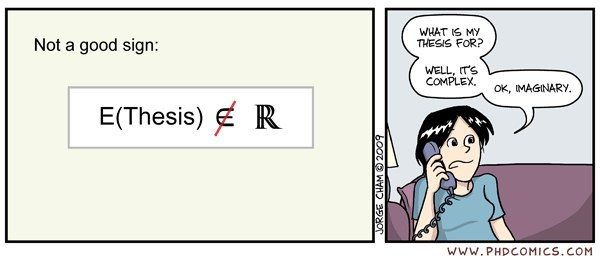
\includegraphics[height=2in]{img/e_thesis_not_in_real.png} \caption{Piled High \& Deeper ~\cite{phd}} \label{fig:img_phd052709s} 
\end{figure}

\cleardoublepage

\special{pdf: out 2 << /Title (Inhaltsverzeichnis) /Dest [ @thispage /FitH @ypos ] >>}

\tableofcontents

\cleardoublepage

% Seitenstil (Fuss- und Kopfzeilen)
\pagestyle{headings} 
\pagestyle{fancy}
\pagenumbering{arabic}


% Werke im Literaturverzeichniss auffhren
% obwohl sie nicht zitiert werden.
\nocite{coanap}
\nocite{aee}
\nocite{wanka}

% section (end)
%%%%%%%%%%%%%%%%%%%%%%%%%  Einfhrung %%%%%%%%%%%%%%%%%%%%%%%%%%%%%
\section{Einfhrung} % (fold)
Approximative Algorithmen sind Algorithmen, die mit schneller\footnote{Schnell ist hier gleichbedeutend mit Polynomzeit} Laufzeit, \emph{nherungsweise} Ergebnisse fr Probleme liefern, fr die bis heute keine Algorithmen mit polynomieller Laufzeit bekannt sind oder existieren solange $\mathbb P \neq \mathbb{NP}$ gilt. Die Besonderheit der \emph{Approximativen Algorithmen} besteht hier in der \glqq Garantie\grqq{} der Gte. Whrend bei \emph{Heuristischen Verfahren} die Qualittsaussagen experimentell u.a. mit Eingaben durch \emph{Benchmark-Mengen} bestimmt werden. Oder den \emph{Parametrisierten Algorithmen} bei denen zwar immer eine optimale Lsung gefunden wird, aber der nicht polynomielle Teil der Laufzeit vorher durch die Parameter eingeschrnkt werden muss.\\
\subsection{Beispiel List Scheduling}

Ein praktisch relevantes Beispiel stellt das Problem \ac{JS} dar:

\begin{example}
	[\textsc{Job Scheduling}] Auf $p$ Prozessoren ($P_1,P_2,...,P_n$) sollen $t$ Tasks ($T_1,T_2,...,T_n$) verteilt werden. Dabei hat jeder Task eine Laufzeit $l_i$, die der Prozessor bentigt, um diesen abzuarbeiten. 
\end{example}

Zustzlich gilt: 
\begin{itemize}
	\setlength{\parskip}{0.5pt}
	\item Angefangene Tasks knnen nicht abgebrochen werden
	\item Ein Prozessor kann zu jedem Zeitpunkt nur einen Task ausfhren
	\item Die Ausfhrungsgeschwindigkeit der Prozessoren ist identisch
\end{itemize}

Gesucht ist dann eine Belegung der Prozessoren, auch Schedule genannt, die alle Tasks mit der kleinsten Gesamtlaufzeit abarbeitet.\\

\begin{example}
	[Prozessorbelegung]\label{prozessorbelegung} 
	Auf einem Rechner mit einem Dual-Core mssen folgende Tasks abgearbeitet werden:\\
	\begin{align}
		\begin{tabular}
			{l|l} \textsc{Task}&\textsc{Zeit}\\
			\hline \hline 1 & 1\\
			\hline 2 & 2\\
			\hline 3 & 2\\
			\hline 4 & 4\\
			\hline 5 & 1\\
		\end{tabular}
	\end{align}
	Die optimale Belegung hierzu wre $((0,P_1),(1,P_1),(3,P_1),(0,P_2),(4,P_2)$  und htte eine Dauer von 5 Zeiteinheiten.
	% \begin{figure}[htbp]
	% \centering 
	% 	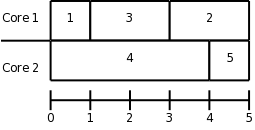
\includegraphics[height=90px]{img/opt_prozessor_belegung.png} \caption{Optimale Belegung von 2 Prozessoren aus Beispiel~\ref{prozessorbelegung}} \label{fig:img_opt_prozessor_belegung} 
	% \end{figure}
\end{example}

Die optimale Belegung lsst sich hier noch durch simples Probieren herausfinden, indem man alle Mglichkeiten durchprobiert und die jeweilige Laufzeit der Belegung notiert.

Eine einfache Implementierung wre der Algorithmus \textsc{Job Scheduling} nach Graham (\cite{gra66} ). Dieser verteilt die Tasks auf den nchsten jeweils gerade frei gewordenen Prozessor. Dies ist zwar am einfachsten zu implementieren, hat aber den Nachteil, dass der Algorithmus die Eingabe als Gesamtes nicht betrachtet.

\label{fig:js}
\begin{algorithm}[h]
\KwIn{$p$ Prozessoren,$t$ Tasks und die Laufzeiten $l_i$ fr jeden Task}
\KwOut{Eine Prozessorbelegung $S$ mit minimalen Makespan}
\caption{\textsc{Job Schedule}}
$S$ = null \;
\For{i = 1 to $p$}
	{$a_i$ = null\;}
\For{k = 1 to $t$}{
	Berechne das kleinste $i$ mit $a_i = min\{a_t;t \in \{1...,p\}\}$\;
	$s_k = a_i$\;
	$a_i = a_i + l_k$\;
	$S = S \cup \{(S_k,P_i)\}\;$}
return $S$\;
\end{algorithm}

Der Makespan des Algorithmus zu Beispiel~\ref{prozessorbelegung} wrde dann wie folgt aussehen:

\begin{figure}[htbp]
	\centering
		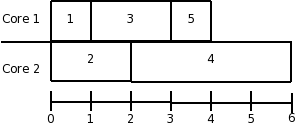
\includegraphics[height=90px]{img/nich_so_opt_prozessor_belegung.png}
	\caption{Nicht ganz so optimale Belegung}
	\label{fig:img_nich_so_opt_prozessor_belegung}
\end{figure}


% (end)
%%%%%%%%%%%%%%%%%%%%%%%%%  Definitionen %%%%%%%%%%%%%%%%%%%%%%%%%%%
\section{Definitionen} % (fold)

Wenn $\Sigma$ Alphabet ist, dann ist $\Sigma^*$ die Menge aller endlichen Folgen von Elementen aus $\Sigma$. Man spricht hier auch von \emph{Wrtern}.\label{Wort} In dieser Definition ist auch die leere Folge, auch leeres Wort genannt, mit eingeschlossen, welche mit $\epsilon$ bezeichnet wird. Siehe auch \cite[S.11]{tikg}

\begin{example}[Binres Alphabet]
	Sei ein Alphabet $\Sigma = \{1,0\}$ gegeben. \\
	So ist $\Sigma^* = \{\epsilon,0,1,00,01,10,11,...\}$.\label{Sigma} 
\end{example}



\begin{definition}[Charakteristische Funktion]
	Die charakteristische Funktion einer Menge $P \subseteq \Sigma^*$ ist $f_P:\Sigma^* \rightarrow \{0,1\}$. Wobei fr alle $w \in \Sigma^*$ gilt:\\
	\begin{align}
		f_{P}(w) = 
		\begin{cases}
			1, w \in P\\
			0, w \notin P			
			% "ist nicht Element von" ist \notin ... Latex kann so einfach sein :D
		\end{cases}
	\end{align}
\end{definition}

Die charakteristische Funktion einer Menge gibt also Auskunft darber, ob ein Wort $w$ in der Menge $\Sigma^*$ enthalten ist. Wie in der Informatik gebruchlich entspricht $1 \triangleq$ \emph{\textbf{Wahr}} und $0 \triangleq$ \emph{\textbf{Falsch}}.


% (end)

%%%%%%%%%%%%%%%%%%%%%%%%%  Probleme %%%%%%%%%%%%%%%%%%%%%%%%%%%%%%%
\subsection{Probleme} % (fold)
\label{sub:probleme} 
Generell kann man zwischen 4 Problemarten unterscheiden:
\begin{description}
	\item[Entscheidungsproblem] Gibt es \emph{m}?
	\item[Suche] Finde den Weg von \emph{l} nach \emph{m}
	\item[Optimierung] Finde den \emph{krzesten} Weg von \emph{l} nach \emph{m}
	\item[Zhlen] Zhle die Wege von \emph{l} nach \emph{m}
\end{description}


\begin{definition}[Entscheidungsproblem]
	Ein (Entscheidungs-)Problem ist eine Menge P $\subseteq \Sigma^*$ fr die, die charakteristische Funktion $C$ halb oder ganz berechenbar ist.
\end{definition}

Siehe auch \cite[S. 122]{tikg}.
\begin{definition}
	[Entscheidungsalgorithmus] Ein Algorithmus $A$ lst ein Entscheidungsproblem $E$ gdw. er fr alle $x\in E_p$ hlt und wenn $x\in Y_p$ gilt der Algorithmus $1$ ausgibt. 
\end{definition}

$I_E$ ist die Menge aller mglichen Eingaben. Und jede mgliche Eingabe $I_E$ fhrt zu einer Antwort $1$ oder $0$ (Wobei $1=$ Ja und $0=$ Nein). Dies ist deshalb wichtig, da aus einem Optimierungsproblem durch eine zustzliche Schranke ein Entscheidungsproblem gemacht werden kann. 


\begin{definition}
	[Optimierungsproblem] Ein \textbf{Optimierungsproblem} $O$ besteht aus einem Quadruppel $O(I_{o},F,w)$: 
	\begin{itemize}
		\item Eine Menge $I_{o}$ bestehend aus einer Menge von Instanzen 
		\item Zu jeder Instanz $i$ aus $I_O$ gibt es eine $F(i)=_{\mathrm{def}}\{\text{Menge \allowbreak aller \allowbreak zulssigen Lsungen}\}$ 
		\item Zu jeder Lsung $L_O$ aus $F(i)$ gibt es einen Funktion $w(L_O)$ die, die Lsung bewertet
		\item Ziel $w \in \{\text{min,max}\}$
	\end{itemize}
\end{definition}
Bei Optimierungsproblemen existieren meist zu einer Eingabe mehrere Lsungen. Hier soll dann abhngig von einem Bewertungskriterium eine Lsung mit minimalen Kosten und maximalen Nutzen gefunden werden.
Bei dem Beispiel des \ac{JS} wren die Instanzen $I$ die Anzahl der Prozessoren (oder Kerne), sowie die abzuarbeitenden Tasks und deren Bearbeitungszeit. $F(i)$ sind alle Schedules mit allen abzuarbeitenden Prozessen. $w$ entspricht hier der Zeit der Bearbeitung aller Jobs und ist zu minimieren (Minimierungsproblem).
\begin{definition}
	[Approximationsalgorithmus] Ein Approximationsalgorithmus fr ein Optimierungsproblem $O$ ist ein Algorithmus der zur Eingabe $I$
	\begin{itemize}
		\item polynomielle Laufzeit hat
		\item eine zulssige Lsung $L_{O} \in F(i)$ berechnet
	\end{itemize}
\end{definition}

%(end)
%%%%%%%%%%%%%%%%%%%%%%%%%  Komplexitt %%%%%%%%%%%%%%%%%%%%%%%%%%%%
\subsection{Komplexitt} % (fold)
Um Algorithmen bewerten zu knnen werden einige Aussagen ber die Laufzeit und Komplexitt bentigt. Der Einfachheit halber messen wir die Laufzeit eines Algorithmus in Instruktionen die abgearbeitet werden msssen bis der Algorithmus terminiert. Dabei entspricht eine Anweisung im Code einer Instruktion im Prozessor. 
\begin{definition}
	[Komplexittsklasse $\mathbb P$] Probleme gehren zur Komplexittsklasse $\mathbb{P}$ gdw. fr sie ein Algorithmus existiert, der sie  unabhngig von der Eingabelnge der Instanzen in polynomieller Laufzeit lst. 
\end{definition}

Auch wenn die Klasse $\mathbb P$ in der Algorithmik als \emph{schnell} gilt. So ist zu beachten, dass ein Algorithmus mit einer Laufzeit von $n^{(2000)}$ sich zwar in $\mathbb P$ befindet aber alles andere als eine kurze Laufzeit hat.

\begin{definition}
	[Komplexittsklasse $\mathbb{NP}$] Eine Sprache $L\subseteq \Sigma^*$ befindet sich in $\mathbb{NP}$, wenn fr sie ein polynomiell beschrnkter Algorithmus A und ein Polynom p existieren, so dass fr alle $x \in \Sigma^*$ gilt:\\
	$x\in L$ genau dann wenn $\exists w$ mit $|w|\leq p(|x|)$so, dass $A(x,w)$ = wahr
\end{definition}
Die Klasse $\mathbb{NP}$ besteht also aus Problemen, fr deren Lsung kein effizienter Algorithmus bekannt ist, die Lsung selber aber in polynomialzeit berprfbar ist.\footnote{
Eine Liste mit NP-Vollstndingen Problemen lsst sich hier finden: \url{http://www.csc.liv.ac.uk/~ped/teachadmin/COMP202/annotated_np.html}} Einen Schritt weiter geht die Klasse $\mathbb{NPO}$, die die Komplexittsklasse der NP der Optimierungsprobleme darstellt. 

\begin{definition}
	[Komplexittsklasse $\mathbb{NPO}$] Ein Optimierungsproblem $O = (I_{o},F,w)$ liegt in der Klasse $\mathbb{NPO}$ gdw.:
	\begin{itemize}
		\item In polynomieller Zeit getestet werden kann ob eine Eingabe auch eine Instanz kodiert
		\item Die Bewertungsfunktion ist in polynomieller Zeit berechenbar
		\item Es exisitieren Polynome $p$ und $q$ so dass fr alle Instanzen $i \in I$ gilt:
		\subitem Fr jede zulssige Lsung $x \in F(i)$ gilt $|x|\leq p(|i|)$
		\subitem Fr jeden String $y$ mit $|y| \leq p(|i|)$ kann in Zeit $q(|i|)$ getestet werden, ob $y \in F(i)$
	\end{itemize}
\end{definition}

\begin{definition}
	[Komplexittsklasse $\mathbb{PO}$] Ein Optimierungsproblem $O$ liegt in der Klasse $\mathbb{PO}$, wenn $O \in \mathbb{NPO}$ liegt und zu jeder Instanz in polynomieller Zeit eine optimale Lsung berechnet werden kann.
\end{definition}
%(end)


%%%%%%%%%%%%%%%%%%%%%%%%%  Gte %%%%%%%%%%%%%%%%%%%%%%%%%%%%
\subsection{Gte}%(fold)

Damit konkrete Aussagen ber die Qualitt der errechneten Ergebnisse gemacht werden knnen, mssen diese mit der optimalen Lsung verglichen werden. Der einfachste Weg ist die Differenz. Je kleiner sie ist desto nher liegt der errechnete Wert am Optimum. Stellt man Aussagen ber diese Art des Vergleichs an, so spricht man von einer absoluten Gte, da das Ergebnis im absoluten Zusammenhang mit dem Optimalen Wert steht.

\begin{definition}[Absolute Gte]
	Sei $\Pi$ ein Optimierungsproblem und $A$ ein Approximationsalgorithmus fr $\Pi$. 
	\begin{itemize}
		\item $A(I)$ hat eine absolute Gte von $\mathcal{AG}_{A}(\mathcal I)=|A(\mathcal I)-\text{OPT}(\mathcal I)|$
		\item $\mathcal{AG}_{A}^{WC}(n) = \text{max}\{\mathcal{AG}_{A}(\mathcal I)|\in \mathcal D,|\mathcal I| \leq \text{n}\}$ ist die \emph{absolute}-worst-case-Gte
	\end{itemize}
\end{definition}

Gilt fr alle n: $\mathcal{AG}_{A}^{WC}(\text{n}) \leq \mathcal{AG}_{A}(n)$ so \textbf{garantiert} $A$ eine absolute Gte von $\mathcal{AG}_{A}(n)$. Man spricht dann von einer \emph{absoluten Gtegarantie}. Solch eine absolute Garantie ist dann sehr praktisch, wenn die Lsungen gro sind. So ist eine absolute Abweichung von 5 bei einem optimalen Wert von 6 mehr oder weniger katastrophal, bei einem optimalen Wert von $100.000$ jedoch praktisch zu vernachlssigen. Ein weitere Mglichkeit ist es die Gte in Relation zum optimalen Wert anzugeben. Man spricht dann von einer relativen Gtegarantie.

\begin{definition}
	[Relative Gte]
	Sei $A$ ein Approximationsalgorithmus fr das Optimierungsproblem $O$
	\begin{itemize}
		\item $A$ hat eine \emph{relative} Gte von
		\begin{align}
			\mathcal{RG}_{A}(\mathcal I)=\text{max}\left\{
				\frac{A(\mathcal I)}{OPT(\mathcal I)},\frac{OPT(\mathcal I)}{A(\mathcal I)}
				\right\}
		\end{align}
		\item  $\mathcal{RG}_{A}^{WC}(n) = \text{max}\{\mathcal{RG}_{A}(\mathcal I)|\in \mathcal D,|\mathcal I| \leq \text{n}\}$ ist die \emph{relative}-worst-case-Gte
	\end{itemize}
\end{definition}

Gilt fr alle $n$ $\mathcal{RG}_{A}^{WC}(n) \leq \mathcal{RG}_{A}(N)$ dann \textbf{garantiert} $A$ eine relative Gte von $\mathcal{RG}_{A}^{WC}(n)$. Die Gte kann demnach in Dezimalzahlen von 0 bis $\infty$ gemessen werden. Wobei 0 dem Optimum entspricht.

Spricht man von einer relativen Gte muss auch der relative Fehler definiert werden:

\begin{definition}[Relativer Fehler]
	Ein Approximationsalgorithmus $A$ hat einen relativen Fehler $\mathcal{RF}$ von
	\begin{align}
		\mathcal{RF}_{A}(\mathcal I) = \frac{|A(\mathcal I)-OPT(\mathcal I)|}{OPT(\mathcal I)} = \left| \frac{A(\mathcal I)}{OPT(\mathcal I)} - 1 \right|
	\end{align}
\end{definition}
%(end)

%%%%%%%%%%%%%%%%%%%%%%%%%  Approximationsklassen %%%%%%%%%%%%%%%%%%
\section{Approximationsklassen} %(fold)
Bisher wurde in den Definitionen davon ausgegangen, dass die Abweichung vom optimalen Wert sich nicht ndert. Allerdings gibt es auch Algorithmen bei denen man sich auf Kosten der Laufzeit  eine kleinere Abweichung \glqq erkauft\grqq{}. Man bergibt dem Algorithmus einen maximal erlaubten Fehler und macht die Laufzeit von jenem abhngig.

\begin{description}
	\item[FPTAS] steht fr \textbf{F}ully \textbf{P}olynomial-\textbf{T}ime \textbf{A}pproximation \textbf{S}cheme und enthlt alle Approximationsalgorithmen deren Laufzeit polynomiell zur Eingabe und zur Gte ist.
	\item[PTAS] steht \textbf{P}olynomial-\textbf{T}ime \textbf{A}pproximation \textbf{S}cheme und enthlt alle Approximationsalgorithmen die sich lediglich zur Gte polynomiell verhlt..
	\item[APX] Alle approximierbaren Algorithmen.
\end{description}

%(end)

%%%%%%%%%%%%%%%%%%%%%%%%%  Beispiel %%%%%%%%%%%%%%%%%%

\section{Beispielanalyse} 
Anfangs wurde das Problem \ac{JS} und folgender Algorithmus dafr vorgestellt:
 
\begin{algorithm}[h]
\KwIn{$p$ Prozessoren,$t$ Taks und die Laufzeiten $l_i$ fr jeden Task}
\KwOut{Eine Prozessorbelegung $S$ mit minimalen Makespan}
\caption{\textsc{Job Schedule}}
$S$ = null \;
\For{i = 1 to $p$}
	{$a_i$ = null\;}
\For{k = 1 to $t$}{
	Berechne das kleinste $i$ mit $a_i = min\{a_t;t \in \{1...,p\}\}$\;
	$s_k = a_i$\;
	$a_i = a_i + l_k$\;
	$S = S \cup \{(S_k,P_i)\}\;$}
return $S$\;
\end{algorithm}

Nun soll die Gte des List Schedule analysiert werden. Seien also \emph{p} Prozessoren gegeben und \emph{t} Tasks die abgearbeitet werden mssen. Dabei seien wie im Algorithmus $s_k$ der Startzeitpunkt, der dem Job vom Algorithmus zugewiesen wurde. $Z$ sei die Laufzeit des gesamten vom Algorithmus erzeugten Schedule. $Z_k = s_k + l_k$ sei der Zeitpunkt an dem der $k$-te Task endet. Des weiteren sei $T_{last}$ der Task der als letztes beendet wird. Daher gilt: $Z_{last} = Z$. Die durchschnittliche Laufzeit des gesamten Schedule betrgt

\begin{align}
	\frac{1}{p} \sum_{k = 1}^{t}  l_{k}
\end{align}

und die durchnittliche Laufzeit jeder Maschine bis zum Startzeitpunkt des letzten Tasks

\begin{align}
	\frac{1}{p} \sum_{k \in \{1,...,t\} \backslash \{last\}}  l_{k}
\end{align}

Es gibt also mindestens eine Maschine, die bis zu diesem Zeitpunkt voll ausgelastet war. Daraus lsst sich schlieen, dass der Startzeitpunkt des letzten Tasks entweder genau auf diesem Punkt liegt oder frher (auf einer anderen Maschine). 

\begin{align}
	s_{last} \leq \frac{1}{p} \sum_{k \in \{1,...,t\} \backslash \{last\}}  l_{k}
\end{align}

So folgt daraus:

\begin{align}
	Z & = Z_{last} \\
	  & = s_{last} + l_{last} \\
	  & \stackrel{\mathrm{(8)}} \leq  \frac{1}{p} \sum_{k \in \{1,...,t\} \backslash \{last\}}  l_{k} + l_{last}\\
	& = 	\frac{1}{p} \sum_{k = 1}^{t}  l_{k} + \left(1 - \frac{1}{p}\right) l_{last}\\
\end{align}

Sei $OPT$ ein Optimaler Schedule so ist $OPT$ $\geq l_{last}$. Des Weiteren gilt: $OPT \geq \frac{1}{p} \sum_{k = 1}^{t}  l_{k}$.

\begin{align}
	& \leq OPT + \left(1 - \frac{1}{p}\right) OPT\\
	& \leq \left(2 - \frac{1}{p}\right)OPT
\end{align}

Damit kann also gezeigt werden, dass der Algorithmus eine \emph{garantierte} Gte von $\left(2-\frac{1}{p}\right)$ hat, wobei $p$ die Anzahl der Prozessoren ist. Die Schwachstelle dieses Algorithmus ist, dass er durch groe Tasks am Ende eine stark unausgeglichene Verteilung erzeugt. Dies knnte durch vorheriges sortieren der Tasks vermieden werden.

\vfill
\bibdata
\vfill 
% Literatur
\cleardoublepage \special{pdf: out 2 << /Title (Literatur) /Dest [ @thispage /FitH @ypos ] >>} 
\def\bibname{Literatur} \addcontentsline{toc}{section}{Literatur} 
\bibliographystyle{literature/plaindin}
%\bibliography{literature/literatur}
\bibliographystyle{alphadin}
\bibliography{approx_lit}



\end{document}

%(end)
